\documentclass{standalone}
\usepackage{tikz}
\begin{document}
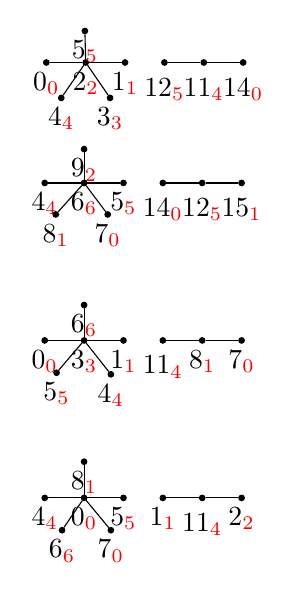
\begin{tikzpicture}[every node/.style={draw, circle, fill=black, minimum size=2pt, inner sep=0pt}]
\node[fill=black, label=below:{\color{black}$0_{\textcolor{red}0}$}] (G1N0) at (3.72,7.33) {};
\node[fill=black, label=below:{\color{black}$2_{\textcolor{red}2}$}] (G1N2) at (4.22,7.33) {};
\node[fill=black, label=below:{\color{black}$1_{\textcolor{red}1}$}] (G1N1) at (4.72,7.33) {};
\node[fill=black, label=below:{\color{black}$3_{\textcolor{red}3}$}] (G1N3) at (4.53,6.88) {};
\node[fill=black, label=below:{\color{black}$4_{\textcolor{red}4}$}] (G1N4) at (3.91,6.88) {};
\node[fill=black, label=below:{\color{black}$5_{\textcolor{red}5}$}] (G1N5) at (4.21,7.73) {};
\node[fill=black, label=below:{\color{black}$12_{\textcolor{red}5}$}] (G1N12) at (5.22,7.33) {};
\node[fill=black, label=below:{\color{black}$11_{\textcolor{red}4}$}] (G1N11) at (5.72,7.33) {};
\node[fill=black, label=below:{\color{black}$14_{\textcolor{red}0}$}] (G1N14) at (6.22,7.33) {};
\draw (G1N2) -- (G1N0);
\draw (G1N2) -- (G1N1);
\draw (G1N2) -- (G1N3);
\draw (G1N2) -- (G1N4);
\draw (G1N2) -- (G1N5);
\draw (G1N12) -- (G1N11);
\draw (G1N11) -- (G1N14);
\node[fill=black, label=below:{\color{black}$4_{\textcolor{red}4}$}] (G2N4) at (3.70,5.80) {};
\node[fill=black, label=below:{\color{black}$6_{\textcolor{red}6}$}] (G2N6) at (4.20,5.80) {};
\node[fill=black, label=below:{\color{black}$5_{\textcolor{red}5}$}] (G2N5) at (4.70,5.80) {};
\node[fill=black, label=below:{\color{black}$7_{\textcolor{red}0}$}] (G2N7) at (4.50,5.40) {};
\node[fill=black, label=below:{\color{black}$8_{\textcolor{red}1}$}] (G2N8) at (3.84,5.40) {};
\node[fill=black, label=below:{\color{black}$9_{\textcolor{red}2}$}] (G2N9) at (4.20,6.23) {};
\node[fill=black, label=below:{\color{black}$14_{\textcolor{red}0}$}] (G2N14) at (5.20,5.80) {};
\node[fill=black, label=below:{\color{black}$12_{\textcolor{red}5}$}] (G2N12) at (5.70,5.80) {};
\node[fill=black, label=below:{\color{black}$15_{\textcolor{red}1}$}] (G2N15) at (6.20,5.80) {};
\draw (G2N6) -- (G2N4);
\draw (G2N6) -- (G2N5);
\draw (G2N6) -- (G2N7);
\draw (G2N6) -- (G2N8);
\draw (G2N6) -- (G2N9);
\draw (G2N14) -- (G2N12);
\draw (G2N12) -- (G2N15);
\node[fill=black, label=below:{\color{black}$0_{\textcolor{red}0}$}] (G3N0) at (3.70,3.80) {};
\node[fill=black, label=below:{\color{black}$3_{\textcolor{red}3}$}] (G3N3) at (4.20,3.80) {};
\node[fill=black, label=below:{\color{black}$1_{\textcolor{red}1}$}] (G3N1) at (4.70,3.80) {};
\node[fill=black, label=below:{\color{black}$4_{\textcolor{red}4}$}] (G3N4) at (4.54,3.37) {};
\node[fill=black, label=below:{\color{black}$5_{\textcolor{red}5}$}] (G3N5) at (3.85,3.39) {};
\node[fill=black, label=below:{\color{black}$6_{\textcolor{red}6}$}] (G3N6) at (4.20,4.25) {};
\node[fill=black, label=below:{\color{black}$11_{\textcolor{red}4}$}] (G3N11) at (5.20,3.80) {};
\node[fill=black, label=below:{\color{black}$8_{\textcolor{red}1}$}] (G3N8) at (5.70,3.80) {};
\node[fill=black, label=below:{\color{black}$7_{\textcolor{red}0}$}] (G3N7) at (6.20,3.80) {};
\draw (G3N3) -- (G3N0);
\draw (G3N3) -- (G3N1);
\draw (G3N3) -- (G3N4);
\draw (G3N3) -- (G3N5);
\draw (G3N3) -- (G3N6);
\draw (G3N11) -- (G3N8);
\draw (G3N8) -- (G3N7);
\node[fill=black, label=below:{\color{black}$4_{\textcolor{red}4}$}] (G4N4) at (3.70,1.80) {};
\node[fill=black, label=below:{\color{black}$0_{\textcolor{red}0}$}] (G4N0) at (4.20,1.80) {};
\node[fill=black, label=below:{\color{black}$5_{\textcolor{red}5}$}] (G4N5) at (4.70,1.80) {};
\node[fill=black, label=below:{\color{black}$6_{\textcolor{red}6}$}] (G4N6) at (3.92,1.39) {};
\node[fill=black, label=below:{\color{black}$7_{\textcolor{red}0}$}] (G4N7) at (4.54,1.39) {};
\node[fill=black, label=below:{\color{black}$8_{\textcolor{red}1}$}] (G4N8) at (4.20,2.26) {};
\node[fill=black, label=below:{\color{black}$1_{\textcolor{red}1}$}] (G4N1) at (5.20,1.80) {};
\node[fill=black, label=below:{\color{black}$11_{\textcolor{red}4}$}] (G4N11) at (5.70,1.80) {};
\node[fill=black, label=below:{\color{black}$2_{\textcolor{red}2}$}] (G4N2) at (6.20,1.80) {};
\draw (G4N0) -- (G4N4);
\draw (G4N0) -- (G4N5);
\draw (G4N0) -- (G4N6);
\draw (G4N0) -- (G4N7);
\draw (G4N0) -- (G4N8);
\draw (G4N1) -- (G4N11);
\draw (G4N11) -- (G4N2);
\end{tikzpicture}
\end{document}
